%=======================================================================================%
\chapter{From Protons to Proteins: Methods to simulate the inside of a cell.}
\numberwithin{equation}{chapter}

\label{chap:methods}

\chapquote{Nature isn't classical, dammit, and if you want to make a simulation of nature, you'd better make it quantum mechanical, and by golly it's a wonderful problem, because it doesn't look so easy.- Richard P. Feynnman}  {}

This chapter is written for somebody who has studied undergraduate physics and now wishes to model biological systems at the molecular level. Care is taken to dive deeper into the mathematical formulations of simulation methods than is conventionally given in introductory texts. Essentially, this is the understanding of simulation techniques I wish I had when I started studying them. An excellent overview which I would recommend as first reading for any new student can be found in an article by Braun et al. \cite{braun2019} followed by \cite{gapsys2020} for statistical rigour and \cite{pohorille2010} for free energy calculations.  

\section{Quantum Mechanics is Not Tractable at the Scale of Biology.}
Living things are made of atoms and atoms themselves are composed of many particles, protons, neutrons and electrons. The motions these constituent particles are governed by quantum mechanics. Unfortunately, performing simulations for the number of atoms involved in proteins and other cellular components at quantum mechanical accuracy is impossible. Hence, we will show how to take the fundamental formulation of atomic interactions in the Schr\"{o}dinger wave equation and apply approximations in order to produce a model which is capable of simulating macromolecular systems at biologically relevant timescales. 

We will gradually integrate upwards, beginning with the interactions in a single atom we will work our way up to a complex macromolecular system with lipids, water, salts and of course, proteins. Ultimately this section rationalises the treatment of atoms as point charges in classical molecular dynamics simulations. 

\subsection{A full quantum mechanical treatment}
Since we are dealing with atoms which are governed by quantum mechanics we must begin our journey upwards with the time dependent form of the Schr\"{o}dinger wave equation. 

\begin{equation}
i\hbar \frac {\partial}{\partial t} \Psi (\textbf{x},t) = \big[ -\frac{\hbar ^2}{2m}\nabla^2 + V (\textbf{x}, t) \big] \Psi (\textbf{x},t) 
\label {schordinger_time_dependent}
\end{equation}

In quantum systems we treat all particles as waves hence the use of the wave function $\Psi (\textbf{x},t)$. The complex amplitude of the wave function $|\Psi (\textbf {x}, t)|^2$ tells us the likelihood of detecting the particle at time $t$ and at place $\textbf{x}$. The term in the brackets correspond to $-\frac{\hbar ^2}{2m}\nabla^2 $, the kinetic energy of the particle with mass $m$ while $V (\textbf{x}, t)$ is an externally applied potential on the system. Given that the left hand term $i\hbar \frac {\partial}{\partial t} \Psi (\textbf{x},t)$ contains a gradient with respect to time, it governs how the wave function will evolve in time.

When the external potential $V$ has no explicit dependence on time, this equation reduces to the familiar time independent form. 

\begin{equation}
	U \Psi (\textbf{x}, t) = \big[ -\frac{\hbar ^2}{2m}\nabla^2 + V (\textbf{x}) \big] \Psi (\textbf{x}, t) = H \Psi(\textbf{x}, t) 
 \end{equation}

Here, $U$ is an eigenvalue of the Hamiltonian operator $H$. Note that the wave function $\Psi (\textbf {x}, t)$ is still allowed to evolve in time. 

In atomic systems there are two types of particles, nuclei which we will denote with the subscript $n$ and electrons denoted by $e$. In order to treat these elements separately we decompose the Hamiltonian of the system into a few components. 

\begin {equation}
H = \underbrace{T_n + U_{n-n}}_{H_n} + \underbrace{T_e +  U_{e-e} + U_{n-e}}_{H_e}
\end {equation}

Where $T_n$ and $T_e$ denote the kinetic energy of the nuclei and electrons respectively. While $U_{n-n}, U_{n-e}, U_{e-e}$ denote the potential energy for interactions between nuclei, between electrons and nuclei and between electrons respectively.

Since the potential terms all describe charged species, they follow Coulomb's law and have the form.

\begin{equation}
	U_{n-n} = \sum_{i>j} \frac{q_e^2 z_i z_j }{|\textbf{R}_i-\textbf{R}_j|},\quad U_{n-e} = -\sum_{i,l} \frac{q_e^2 z_i }{|\textbf{r}_l-\textbf{R}_i|},\quad  U_{e-e}  = \sum_{l>k} \frac{q_e^2 }{|\textbf{r}_l-\textbf{r}_k|}
\end{equation}

Here the $z_i$ represent the atomic number (and thus the charge) of the $i$th nucleus and $q_e$ is the unit charge of the electron. The reason for the separate coordinates $R_i$ and $r_l$ is to separate out the treatment of nuclei and electrons which will be important once we apply the Born-Oppenheimer approximation.

Meanwhile, the kinetic energy terms are of the form 

\begin {equation}
T_n = - \sum_i \frac{\hbar^2}{2M_i} \nabla_i ^2,\quad  T_e = - \sum_l \frac{\hbar^2}{2m_e} \nabla_l ^2
\end {equation}

$M_i$ represents the mass of the $i$th nucleon and $m_e$ represents the mass of an electron. The operator $\nabla^2 = \frac{\partial^2}{\partial x^2} + \frac{\partial^2 }{\partial y^2} + \frac{\partial^2}{\partial z^2} $. The separate subscripts $i$ and $l$ are due to the different coordinates which we use to denote the positions of the nuclei and the electrons. The reason for this will become clear when we derive the Born-Oppenheimer approximation to separate the wave functions and treat them separately.

\subsection{The Born-Oppenheimer approximation.}
\label{born-oppenheimer}
In order to reach the Born-Oppenheimer approximation we start with the observation that electrons have a mass 3-4 orders of magnitude smaller than the nuclei. This motivates two simplifications. The ``clamped nuclei assumption" where we solve the Schr\"odinger equation whilst nuclei are fixed in space and do not move. And a related assumption known as the ``adiabatic assumption" which postulates that the electrons will respond instantaneously to any changes in the positions of the nuclei. Combining these physical approximations we derive the ``Born-Oppenheimer approximation" for the Schr\"odinger equation which can be used to simplify calculations involving several atoms at once. 

We begin the derivation by examining the time-independent form of the electronic Schr\"odinger wave equation where the nuclei are fixed at positions $R_i$. 

\begin{equation}
	H_e(\bold{r}_l, \bold{R}_i)  \psi_e (\bold{r}_l,\bold{R}_i)  = U_e(\bold{R}_i) \psi_e (\bold{r}_l,\bold{R}_i) 
\end{equation}

Fixing the nuclei in this way gives the ``clamped nuclei" approximation \cite{sherrill}. To solve the wave function for the whole system $\Psi_{tot}$ we use an \textit{ansatz} which decomposes the wave function with an electronic basis into two components: $({\psi_e})_k$ and $({\psi_n})_k$ which are the $k$th eigenfunction solutions to $H_e$ and $H_n$ respectively.

\begin{equation}
	\Psi_{tot} (\bold{r}_l,\bold{R}_i, t) = \sum_{k=0}^\infty {\psi_e}(\bold{r}_l, \bold{R}_i)_k\ {\psi_n}(\bold{R}_i)_k
\end{equation}

Note that there is an implied direct product between the wave functions $\psi_e(\bold{r}_l, \bold{R}_i)$ and $\psi_n(\bold{R}_i)$. When we substitute this expression into the full Schr\"odinger equation \ref{schordinger_time_dependent} we find the following expression for the $k$th nuclear eigenfunction \cite{miller1976} 

\begin{equation}
	i \hbar \frac{\partial} {\partial t} {\psi_n(\bold{R}_i)}_k = \Big[- \sum_i \frac{\hbar^2}{2M_i} \nabla^2_i  + {U_e} (\bold{R}_i)_k\Big] \psi_n (\bold{R}_i)_k + \sum_j C_{kj} \ {\psi_n(\bold{R}_i)}_j 
	\label{adiabatic_approx}
\end{equation}

Where we have coupled the electronic wave functions to each other with the operator 

\begin{equation}
	C_{kj} = \int ({\psi_e})_k ^* \Big[\sum_i\frac{\hbar^2}{2M_i}\nabla^2_i\Big] ({\psi_e})_j d\bold{r}  + \frac{1}{M_i}\sum_{i}\bigg[ \int({\psi_e})_k ^* [-\hbar i \nabla_i]({\psi_e})_jd\bold{r}\bigg] [-\hbar i \nabla_i]
\end{equation}

Using the ``adiabatic assumption" \cite{miller1976} the off-diagonal terms of $C_{kj}$ can be set to $0$. This completely decouples the wavefunction into two components 
\begin{equation}
	\Psi_{tot} (\bold{r}_l,\bold{R}_i, t) = {\psi_e}(\bold{r}_l, \bold{R}_i)_k\ {\psi_n}(\bold{R}_i,t)_k
\end{equation}

Since all cross terms from the direct product can be ignored. With the further assumption that the diagonal terms $C_{kk}$ can also be ignored because they are 4 orders of magnitude smaller than the other terms in \ref{adiabatic_approx} \cite{sherrill}.

We now write the Born-Oppenheimer approximated wave equation for an atomic system.  


\begin{equation}
	i\hbar \frac{\partial}{\partial t} \psi_n(\bold{R}_i)_k = \big[ -\sum_i \frac{\hbar^2}{2M_i} \nabla^2_i + U_e(\bold{R}_i)_k\big] \psi_n(\bold{R_i})_k 
\end{equation}

By rearranging this equation and taking derivative we can see how to use Newton's equations of motion to calculate the forces on the nuclei from the surrounding electric potential 

\begin{equation}
	M_i \ddot{\bold{R}}_i (t) = -\nabla_i U_e (\bold{R_i})
	\label{Newtons_equations}
\end{equation}

By choosing an appropriate time-step one can simply iteratively solve this equation of motion to understand the dynamics of an atomic system. The nuclei will move according to their relative positions to each other and the electron clouds will rearrange in response to that motion. There is no need to calculate the interactions between the nuclei and the electrons. This is sufficient accuracy to simulate the low energy motions of molecules such as the environment found in biological systems. 
%\begin{equation}
%	(H_n + H_e + V_{n-e})  (\psi_e (\bold{r}_l,\bold{R}_i) \psi_n(\bold{R}_i)) =  (E_n  + U_e)(\psi_e (\bold{r}_l,\bold{R}_i) \psi_n(\bold{R}_i) ) 
%\end{equation}
%

%disregard $T_e$, $V_{n-e}$ and $V_{e-e}$ as they will be close to 0 compared to $T_n$ and $V_{n-n}$.

%In the case of hydrogen we lose an order of magnitude so the approximation is less valid, especially at room temperature. CITATION NEEDED


%
%\begin {equation}
%\Psi(R_i,t) = \psi_e (r_l,R_i) \psi_n(R_i,t)
%\end {equation}
%
%The BO assumption means that we can neglect the cross terms from this separation and treat each wave function independently.
%
%\begin {equation}
%T_n + T_\Psi(R_i,t) = \psi_e (r_l,R_i) \psi_n(R_i,t)
%\end {equation}


\section{Classical MD, Molecular Motions Without Quantum Mechanics}
The Born-Oppenheimer approximation gives rise to Hartree-Fock methods and density functional theory (DFT). These more sophisticated physical methods allow us to simulate the organisation of electron clouds around small molecules, finding broad applications in chemistry and materials science \cite{vanmourik2014}. These methods are known as \textit{ab initio} MD. We can derive the energy profile of certain degrees of freedom within the molecule such as the energetics of stretching out a bond or twisting a dihedral angle. These can be useful when designing novel materials. 

However, even with these approximations simulating a large number of atoms is still not computationally tractable. State of the art DFT methods can only simulate on the order of $10^3$ atoms \cite{luo2020} and scales as $O(N^3)$ \cite{kresse1996}. This is not sufficient to simulate proteins and their surrounding solvation environment where the molecular system is usually on the order of $10^4-10^6$ atoms. So, we must use another round of approximations to reach the spatial and time scales necessary to simulate biological molecules. We do this by creating a set of mathematical functions to simplify the calculations further. Here we use a set of virtual springs and other simple models for the energetic interactions between atoms. This creates what's known as an effective potential. 


The CHARMM effective potential employed in this work is similar to those found in all common all-atom molecular dynamics forcefields. The same  functional forms are used in other forcefields such as AMBER, GROMOS and OPLS but with different parameters and design philosophies\cite{lemkul2020}. 

This formulation gives us classical molecular dynamics, sometimes referred to as molecular mechanics (MM). The aim of the classical forcefields discussed here is to use \textit {ab initio} MD as a target for approximation and then refine the parameters to better match experimental quantities. This is discussed in detail in section \ref{forcefields_review}.

We split up the molecular mechanics potential into several components dealing with the energies from covalent bonds, including bond stretching, twisting and bending as well as contributions associated with the forces that atoms exert on each other when they are not bonded together 

\begin{equation}
	U_{MM} = \underbrace{U_{LJ} + U_{Coulomb}}_{U_{non-bonded}} + \underbrace{U_{bonds} + U_{angles} + U_{dihedrals} + U_{impropers}}_{U_{bonded} }
	\label{CHARMM_effective_potential_eq}
\end{equation}

Interestingly, the bonded terms may all reasonably be approximated by harmonic springs

\begin{equation}\label{bonded_eqs}
	\begin{aligned}
	U_{bonded} = \sum_{bonds} k_{b} (b-b_0)^2 + \sum_{angles} k_\theta(\theta-\theta_0)^2+ \sum_{Urey-Bradley} k_u(r_{UB}-r_{UB_0})^2   \\ + \sum_{dihedrals} k_\varphi (1+\cos(n \varphi - \delta)) + \sum_{improper-dihedrals}  k_{\phi} (\phi - \phi_0)^2.
\end{aligned}
\end{equation}

Here, the $k_i$ terms correspond to the strength of the harmonic restraint for a parameter. The $0$ subscript denotes the equilibrium position for that parameter. Even though this formulation is quite simple, it has empirically been shown to be a reasonable approximation for the potential energy functions of quantum mechanics in covalently bonded chemical species. Examples can be seen in figure \ref{QM_MM_compared}.

\begin{figure}
	\begin{center}
	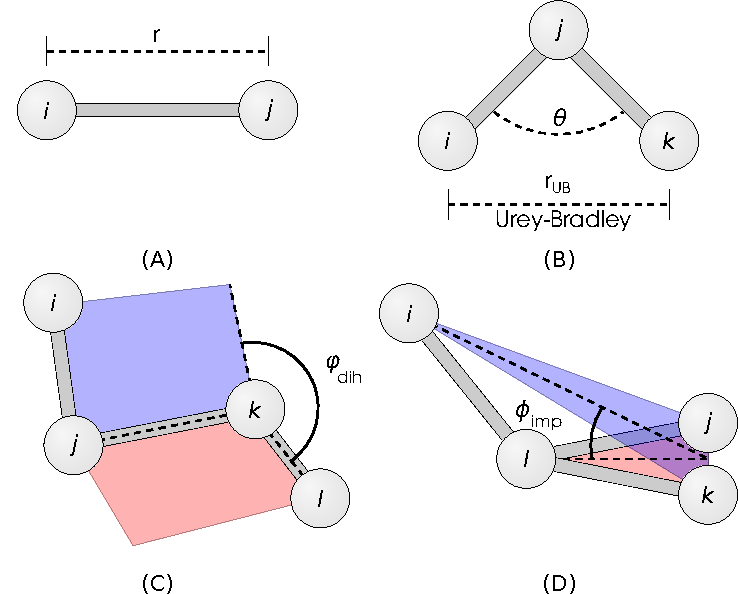
\includegraphics[width=10cm]{figures/bonded_interactions.pdf}
	\end{center}
	\captionsetup{singlelinecheck = false, justification=raggedright}
	\caption[The Bonded Interactions Calculated In Classical Forcefields]{\textbf{The Bonded Interactions Calculated In Classical Forcefields.}}{
	(A) The energy of Bond Stretching is approximated as a harmonic oscillator with respect to their separation $r$. (B) Angles between neighbouring covalently bonded atoms are also approximated as a harmonic oscillator with respect to the angle $\theta$. In some forcefields such as CHARMM there is a correction term for these angular interactions known as Urey Bradley forces. This is calculated using the separation between the non-bonded atoms $i$-$k$ in the triplet with the parameter $r_{UB}$. (C) The dihedral angle between four atoms is calculated by constructing two planes. Each plane is constructed to contains three of the four atoms in the set. One plane encompasses atoms $i, j$ and $k$ here colored in blue and the other plane contains the $j$, $k$ and $l$ atoms colored in red. The dihedral angle is then calculated by taking the angle between these two planes along the line they intersect, the line formed by the $j$-$k$ bond. (D) The improper dihedral angles enforce the planarity of a molecular configuration. A plane is constructed to contain the $i$, $j$ and $k$ (blue) atoms and another plane is constructed to contain the $j$, $k$ and $l$ atoms (red). The improper angle is then calculated as the angle between these two planes. }
	\label{charmm_bonded}
\end{figure}


The term $U_{non-bonded}$ captures interactions which arise when atoms are not covalently bound to each other. Namely, Coulomb forces due to electric charges on the atom, attractive Van Der Walls interactions and repulsion due to Pauli Exclusion the latter two forces are combined into one term, $U_{Lennard-Jones}$, which we will analyse in detail 
\begin{equation}\label{nonbonded_eqs}
	\begin{aligned}
		U_{non-bonded} = \underbrace{\sum_{i>j} \epsilon_{ij} \Big( \Big(\frac{\sigma_{ij}}{r_{ij}}\Big)^{12} - \Big(\frac{\sigma_{ij}}{r_{ij}}\Big)^{6} \Big)}_{U_{Lennard-Jones}} - \underbrace{\sum_{i>j} \frac{q_i q_j } {r_{ij}}}_{U_{coulomb}}
	\end{aligned}
\end{equation}


The $\sigma$ parameter denotes the location of the local minima in the Lennard-Jones potential. This is the optimum distance that two atoms will rest against each other in the absence of other effects. The $\epsilon$ parameter denotes the depth of the potential well, or how stable the two atoms will be in the minimum energy configuration. This is very important for certain physical parameters such as osmotic pressure  \cite{yoo2018a}

Conversely, the partial charges in a system have the greatest influence on the solvation energy.

By focussing on these two physical parameters we can isolate and improve the non-bonded parameters.

\begin{figure}
	\begin{center}
	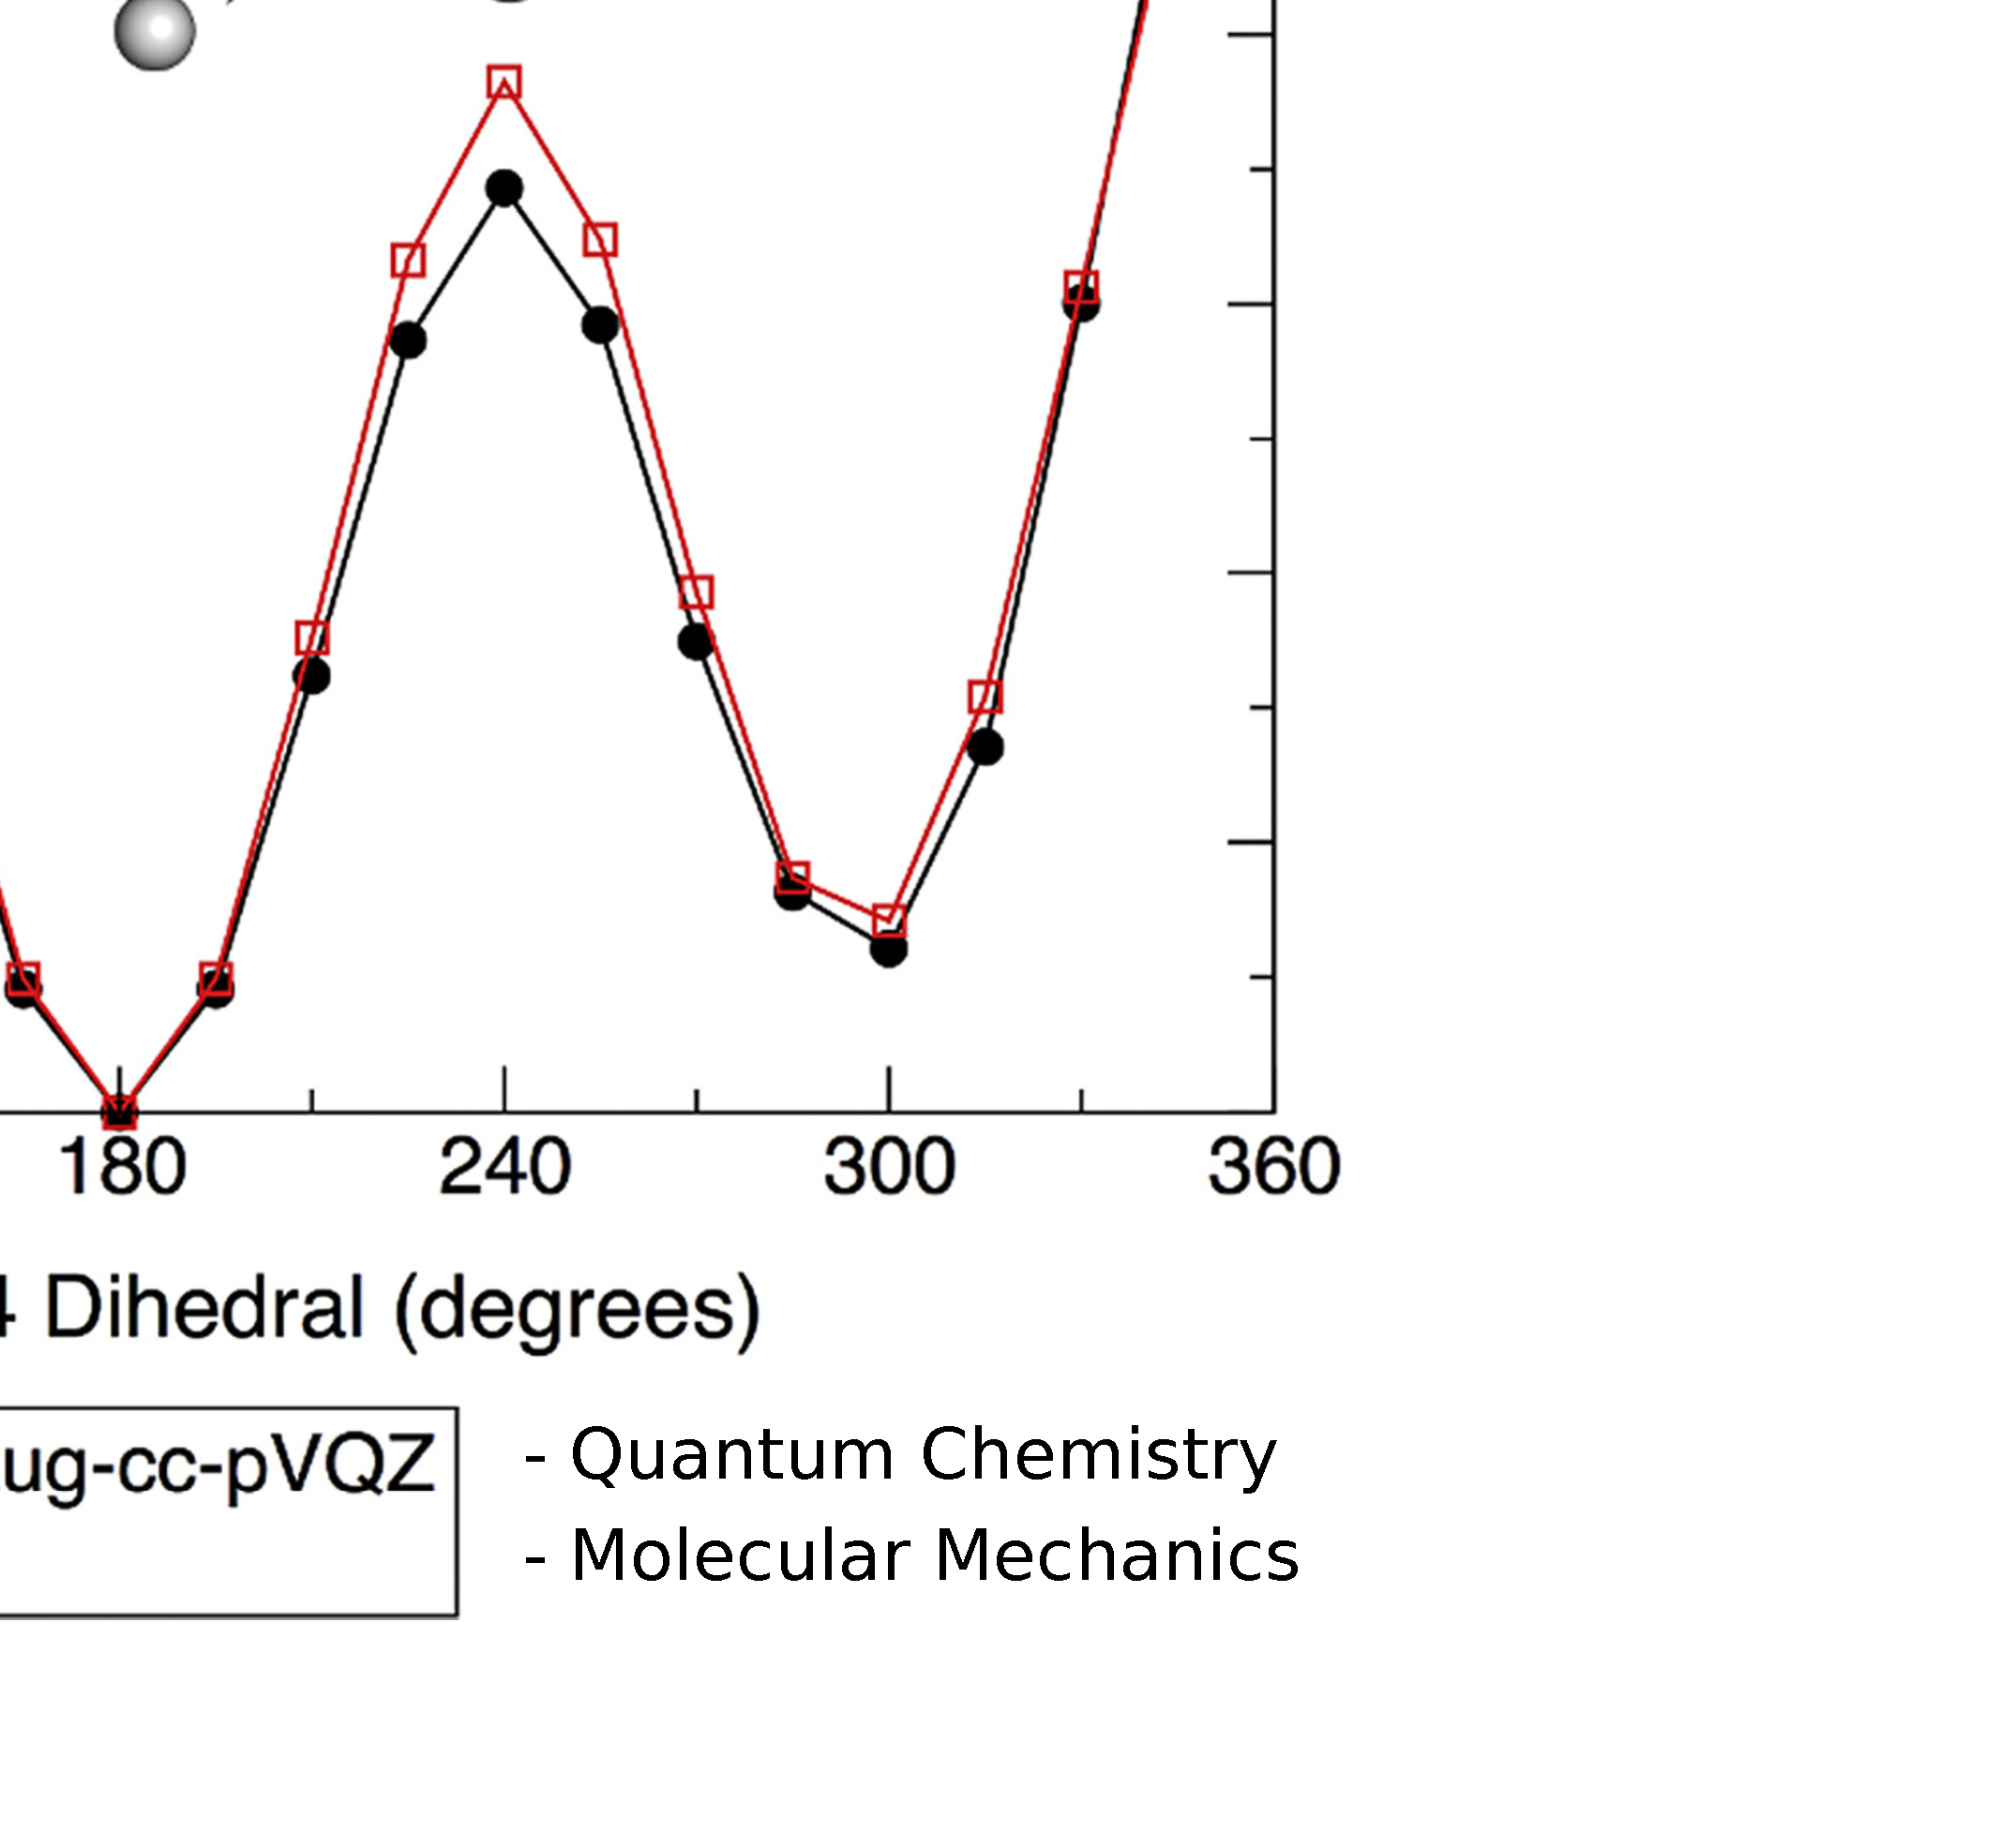
\includegraphics[width=\textwidth]{figures/QM_MM_compared.pdf}
	\end{center}
	\captionsetup{singlelinecheck = false, justification=raggedright}
	\caption[Comparison Between Potentials in Quantum and Classical Forcefields] {\textbf{Comparison Between Potentials in Quantum and Classical Forcefields}}{ A) The Morse potential was formulated to approximate the potential the potential energy surface associated with the stretching of covalent bonds (blue). At low temperatures (the ground state, $v=0$) like those found in classical MD there is good agreement between the Morse potential and the harmonic oscillator (green). Credit Mark Somoza 2006 B) Here the potential of the dihedral angle between the atoms C1,C2,C3 and C4 in a butane molecule is calculated using two methods: Quantum Chemical calculations and approximations using the functional form in \ref{bonded_eqs} \cite{lemkul2020}. Note how the appropriate choice of $k_\varphi$, $n$ and $\delta$ have closely approximated the results the more accurate quantum mechanical calculations.}
 
	\label{QM_MM_compared}
\end{figure}

\subsubsection{The Lennard-Jones Potential}
\begin{figure}
	\begin{center}
		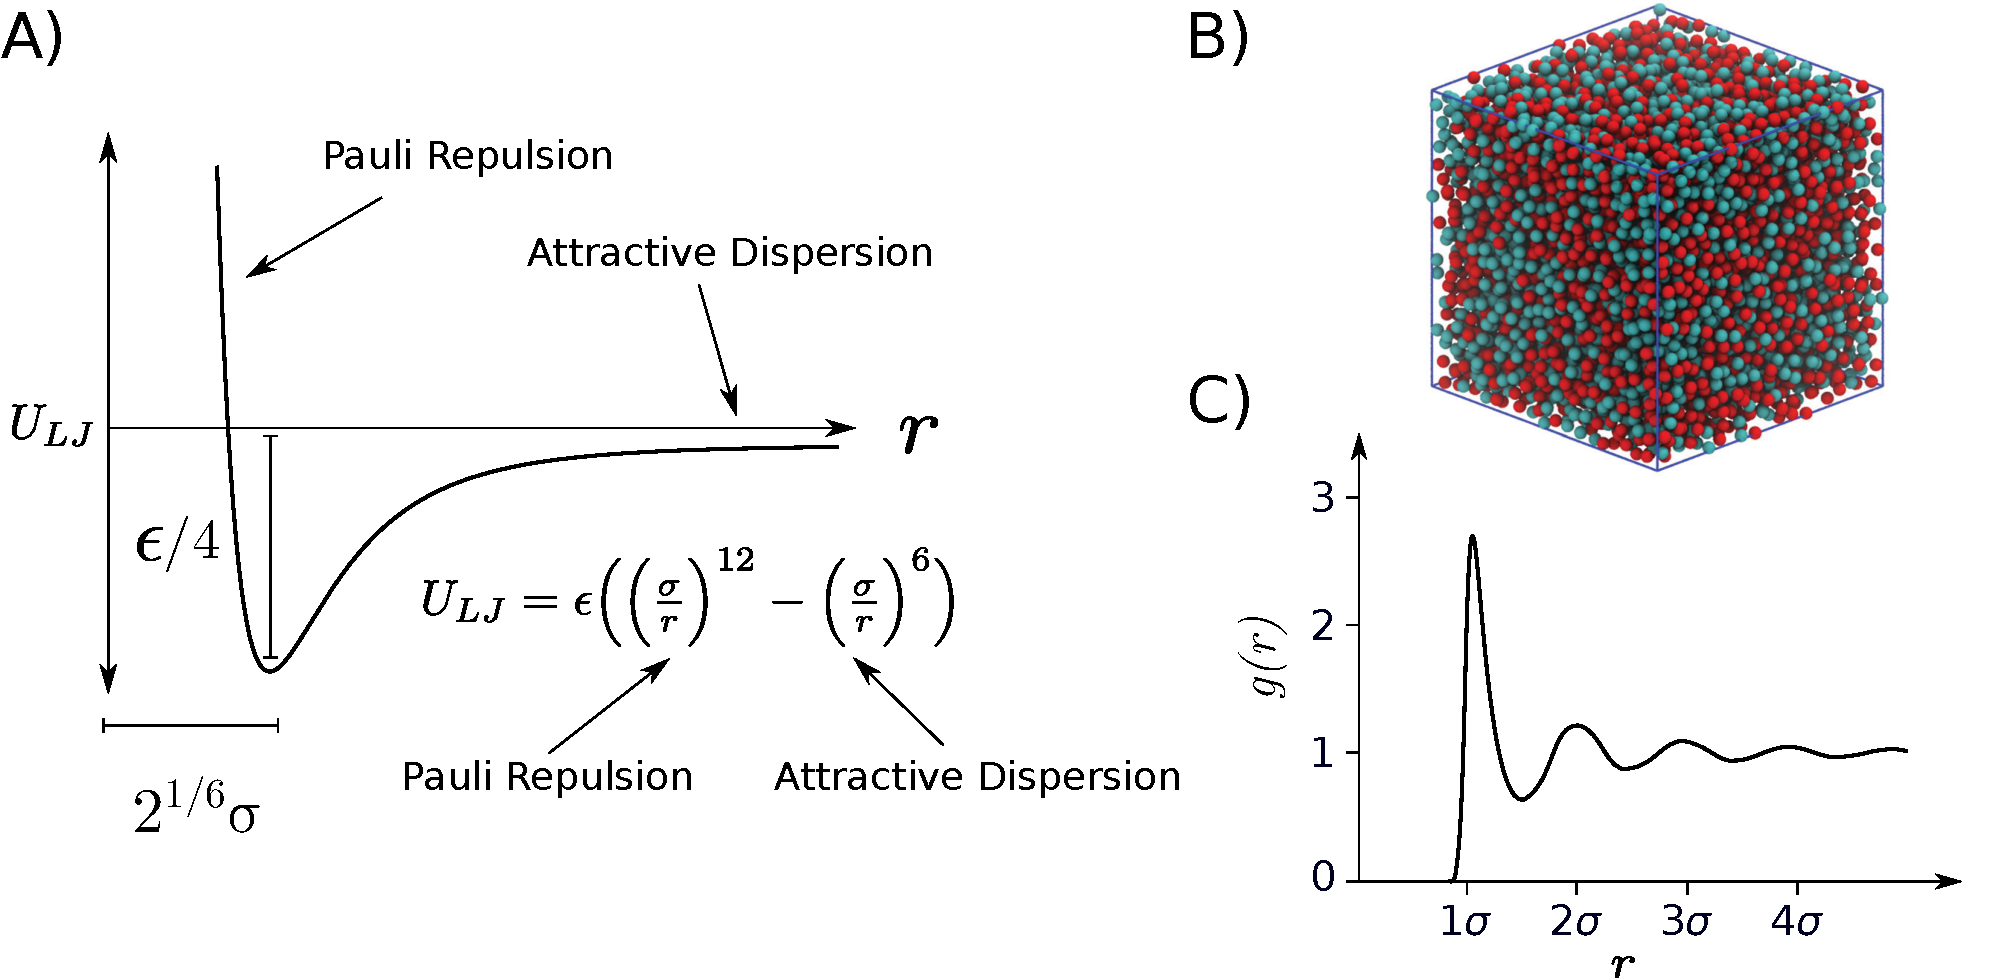
\includegraphics[width=\textwidth]{figures/LJ_figure.pdf}
	\end{center}
	\captionsetup{singlelinecheck = false, justification=raggedright}
	\caption[The Lennard-Jones Potential] {\textbf{The Lennard-Jones Potential}}{A) The Lennard-Jones potential function has two regimes, the far region one dominated by attractive dispersion forces and the close region dominated by repulsion. In the case of atomic systems this is due to the Pauli exclusion principal. B) An example of a fluid modelled with Lennard-Jones particles \cite{chari2019}. C) The radial distribution function ($g$) for a Lennard-Jones fluid \cite{morsali2005}. Note that the peaks in the distribution are spaced roughly 1 $\sigma$ apart. }
	\label{Lennard-Jones_figure}
\end{figure}

\subsection{Philosophy of Different Molecular Mechanics forcefields.}
\label{forcefields_review}
At the time of writing, the four popular forcefields for the simulation of biomolecules are: AMBER, CHARMM, GROMOS and OPLS. Each of these have a slightly different philosophy in their formulation. They may be bottom up, as in the case of AMBER and CHARMM or top down, in the case of OPLS and. Bottom up forcefields take the results from quantum \textit{ab initio} calculations and approximate them with the functional form mentioned above. Conversely, top down forcefields take experimental measurable such as Osmotic pressure, solvation energy. Ultimately, the results from \textit{in silico} experiments must match those of wet lab experimetns so the development of all forcefields has elements of both philosophies. All forcefields assign the partial charges to atoms using the results of \textit{ab initio} QM calculations. The rest of the parameters parameters are derived with other methods. For example, the Lennard-Jones parameters $\sigma$ and $\epsilon$ can be chosen to reproduce calculations of the osmotic pressure from solvated ions \cite{yoo2018a} or dihedral parameters can be chosen to reproduce known secondary structure characteristics of pepteides\cite{huang2017}. Different forcefields have different methods of deriving their parameters. Below is a short summary of the philosophy for the 4 major forcefields taken from the review by Justin Lemkul \cite{lemkul2020} which has an indepth discussion of the history of the development of each of these forcefields.

\begin{itemize}
	\item CHARMM: An all atom forcefield which takes the most inspiration from quantum mechanical calculations. The QM optimized geometries are compared to that found in the geometry taken in the MD simulation in addition to attempts to match molecular dipole moments and rotational energy profiles from QM calculations are also compared to the results from the classical forcefield. An example can be seen in \ref{QM_MM_compared}. Macroscopic experimental quantities may also be used to validate parameters such as solvation energies, crystal geometries, heats of vaporization and sublimation for solids, enthalpy of vaporization and conformational sampling of biomolecules\cite{huang2017}. This is probably the most popular forcefield for the simulation of biomolecules because of of its considerably library of supported compounds especially when combined with its generalised version CGENFF \cite{vanommeslaeghe2010}. 
	\item AMBER: An all atom forcefield which is validated based on its agreement with experimental data such as solvation free energies, crystallographic geometry as well as conformational energies from \textit{ab initio} QM calculations. Similar to CHARMM 

		This forcefield has become the favorite for the simulation of disordered proteins due to its agreement with experimental quantities such as radius of gyration \cite{robustelli2022}\cite{robustelli2018}.

		There is also a generalised version of the AMBER forcefield known as GAFF \cite{wang2004}\cite{wang2006}. Comparisons between generalised forcefields can be found in \cite{zhu2019}.

	\item OPLS: An all atom forcefield. The OPLS forcefield takes the philosophy that since many biomolecules share similar geometries to certain organic liquids, macromolecules can be accurately parameterised by creating a forcefield which correctly reproduces the experimental measurements for these species. Parameters are derived to accurately reproduce the liquid density of certain organic liquids. These parameters are then used as roots to construct larger biomolecules. This method is sometimes used to refine specific in other forcefields \cite{huang2017}.


	\item GROMOS: A united atom forcefield where hydrogen atoms are typically merged into the heavy atom they are bound to, so they are not explicitly treated. Charge assignment is done with DFT. Interstingly, GROMOS uses a quartic form of the bond stretching term 
		\begin{equation}
			U_b = \frac{1}{4} k_b (b^2-b^2_0)^2
		\end{equation}

		Parametrised with enthalpy and liquid densities.

\end{itemize}
Some forcefields share common design philosophies. For example CHARMM and AMBER both manipulate molecular dipole moments in order to account for the presence of polar water water molecules during a classical simulation, while the \textit{ab inito} calculations are often done in a vacuum.


\section{Periodic Boundaries to Simulate the Inside of Cell}
\begin{figure}
	\begin{center}
		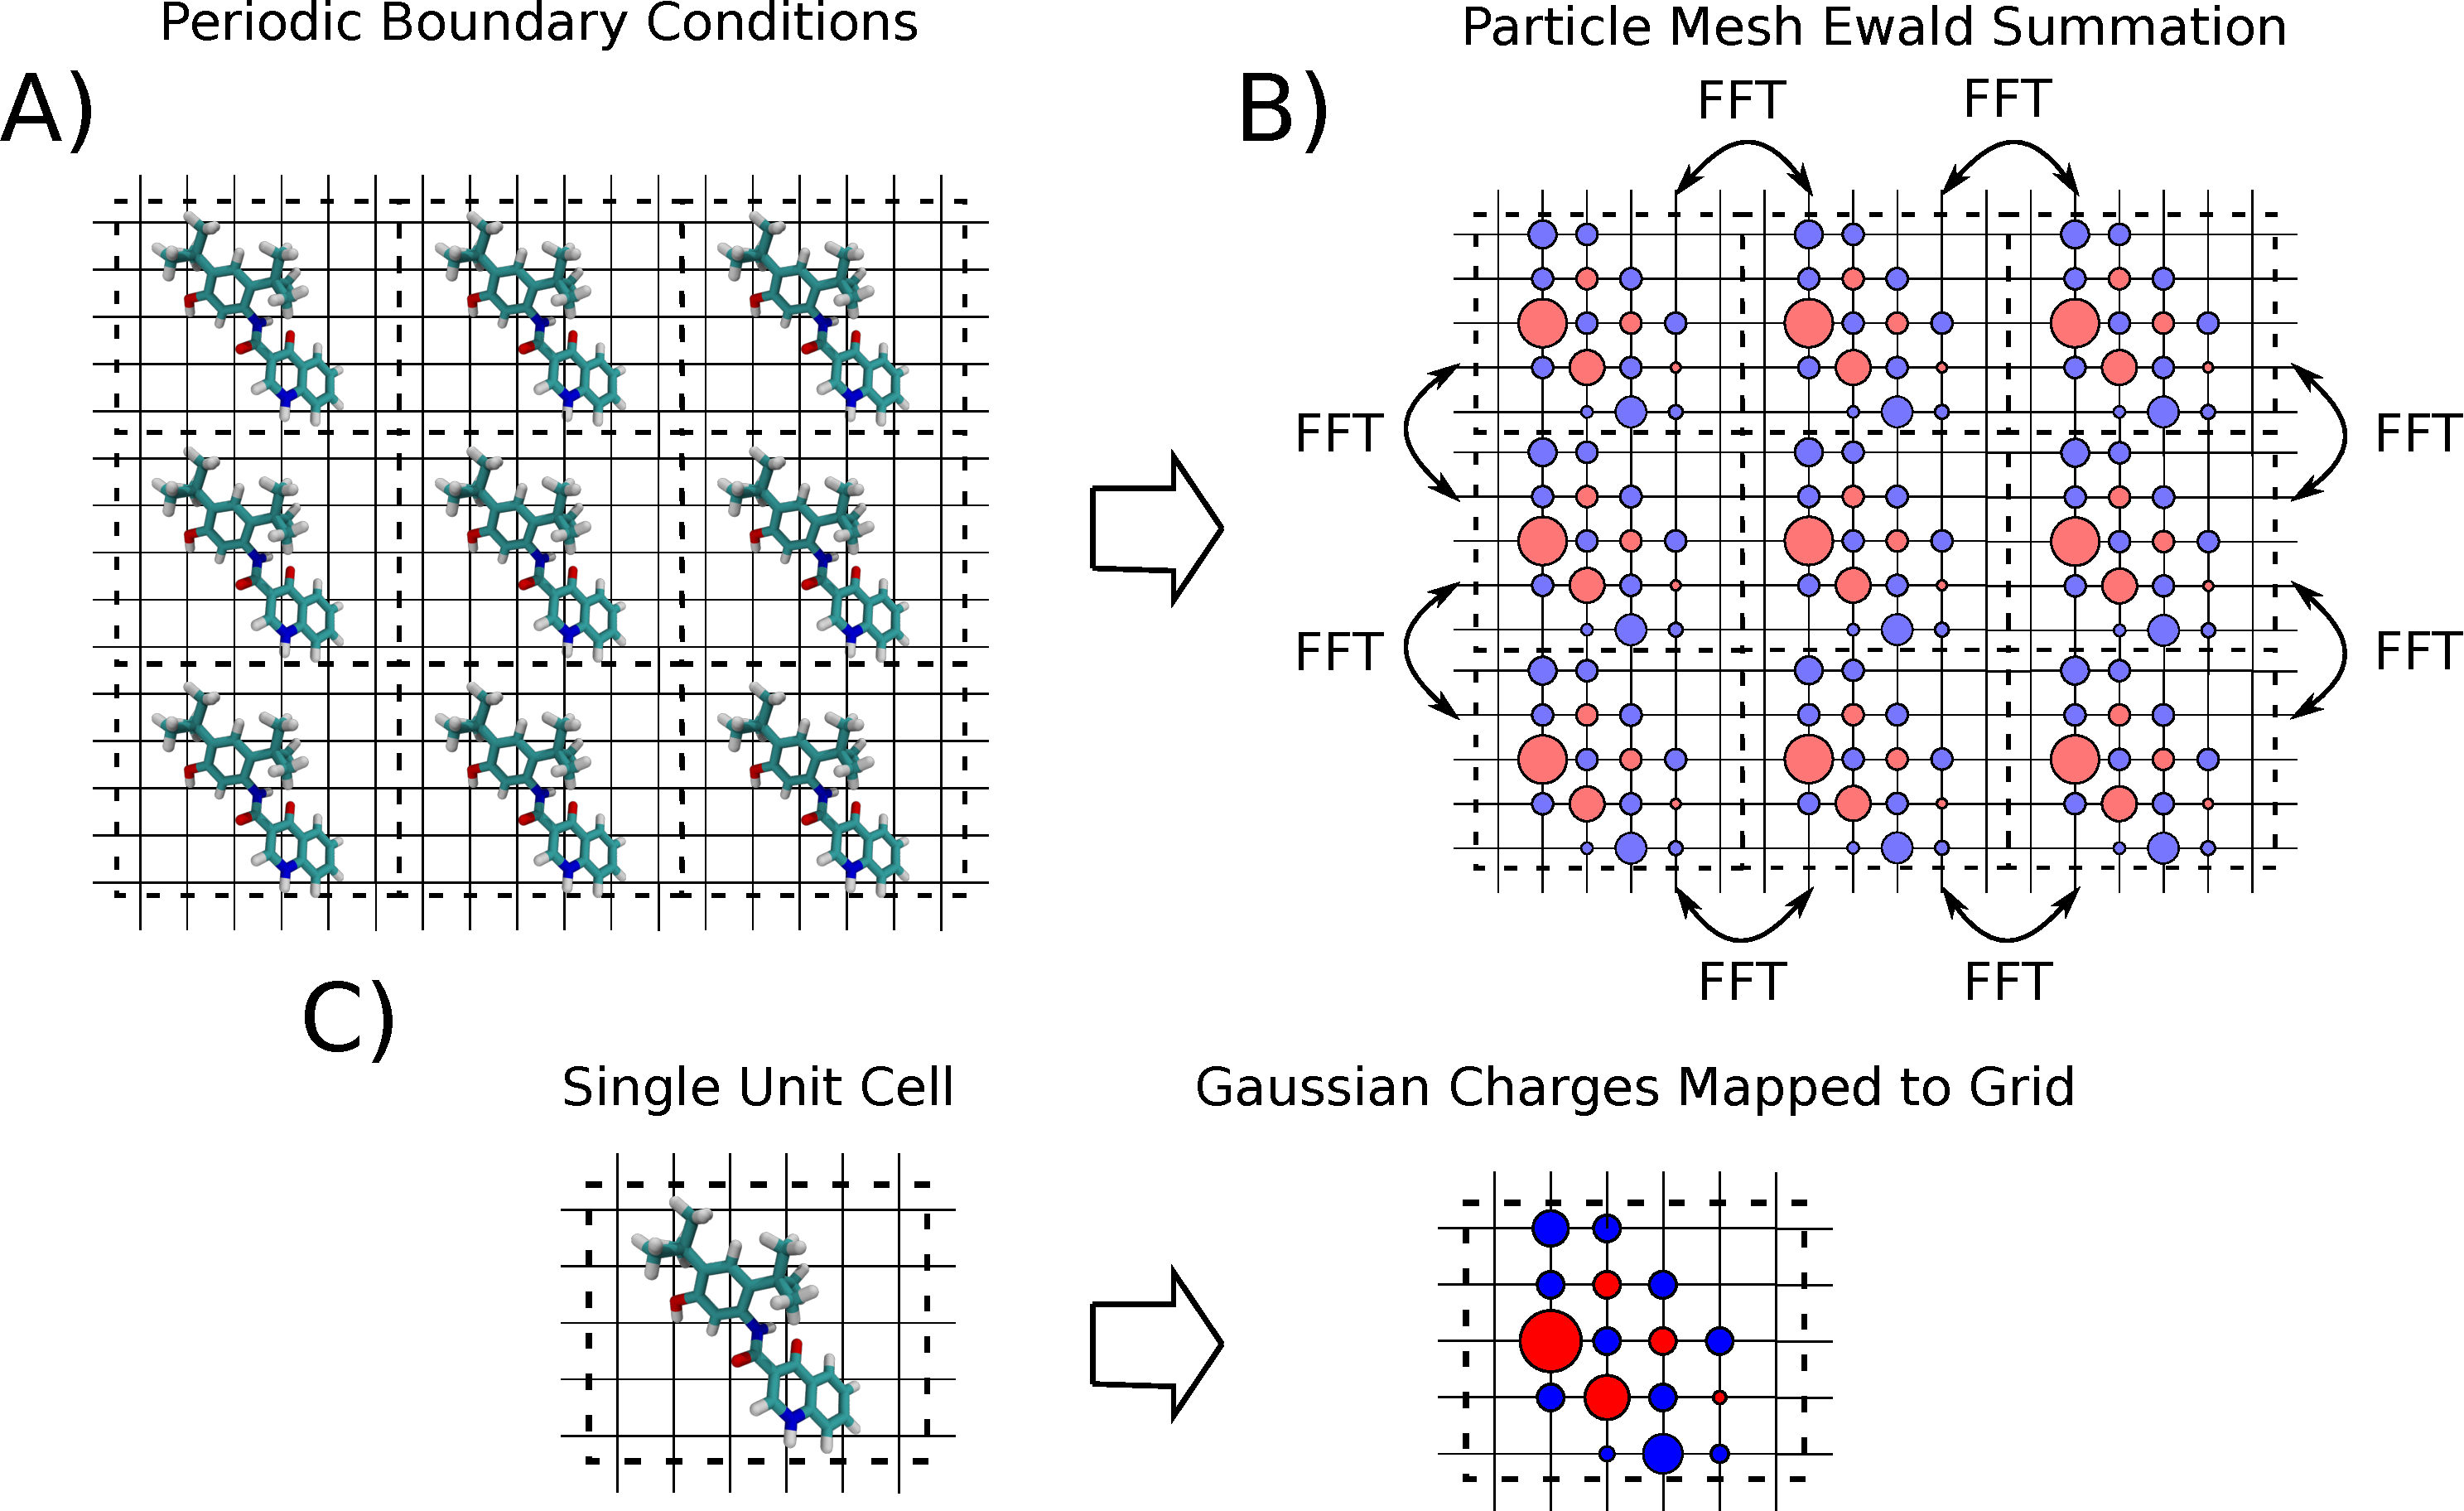
\includegraphics[width=\textwidth]{figures/PME_miro.pdf}
	\end{center}
	\captionsetup{singlelinecheck = false, justification=raggedright}
	\caption[Particle Mesh Ewald Summation] {\textbf{Particle Mesh Ewald Summation}}{A)The molecular system is repeated infinitely along all axes, when atoms reach the edge of the simulation box they are allowed wrap around to the other side of the box. B) The charges in the infinite periodic system are approximated as Gaussian functions on a grid. Then the potential on these screening charges is calculated via a Fast Fourier Transform (FFT). C) A more detailed view of the charge mapping procedure. The point charges in the system are interpolated onto the grid using B-spline interpolation. }
	\label{PME_illustration}
\end{figure}

Inside cells, proteins are immersed in a large solvation environment composed of water and salts \cite{phillips2012}. In order to avoid artefacts we have to replicate this environment somehow\cite{ross2018}. We could make a simulation box large enough to replicate the behavior of a bulk solvent, but even with a large simulation box we can still observe artifacts associated with the vacuum at the boundaries \cite{gapsys2020}. So, to avoid these boundary effects we use periodic boundary conditions (PBCs), allowing atoms to move between images in the simulation box \ref{PME_illustration}. This replicates the molecular system infinitely in every direction. 

Using PBCs might remove vacuum from our molecular system but now we have a different problem. Effectively, with the PBCs, we have created a system with an infinite number of atoms. We have to somehow limit the number of computations we perform. We could simply truncate the calculation of interactions $U_{non-bonded}$ after a certain cutoff distance. This is not an issue for $U_{LJ}$ because the $1/r^6$ and $1/r^{12}$ terms in \ref{Lennard-Jones_figure} decay very quickly for large $r$. Inaccuracies due to this approximation can be further ameliorated with the use of a smooth switching function \cite{klauda2007}\cite{venable2009}. On the other hand, the $1/r$ dependence in $U_{coulomb}$ scales much more slowly so truncating it leads to many artefacts in the simulation.\cite{auffinger1995}\cite{perera1995}\cite{roberts1994}\cite{delbuono1996}\cite{essmann1995}. Note that this periodicity requires that the unit cell is neutral, else the contribution of potential energy from $U_{coulomb}$ will be infinite, leading to artifacts \cite{hub2014}.

To avoid these artefacts and limit computational intensively of our calculations we use a clever scheme known as Particle Mesh Ewald Summation. Interestingly, this scheme ends up scaling better than the pairwise summation in equation \ref{nonbonded_eqs} might imply. The direct summation scales with computational complexity of $O(N^2)$  with the number of atoms while the infinite PME scheme scales as $O (N\log N)$ \cite{darden1993}, though there are some further considerations for large systems on parallel architectures \cite{hardy2015}. Even with these sophisticated algorithms, the calculation of electrostatic potential still represents the largest computational bottle-neck in classical MD \cite{hardy2015}.

For a detailed review of different Particle Mesh Ewald Summation methods and the mathematics behind the method see \cite{shan2005}. A brief outline of the Smooth Particle Mesh Ewald summation is given below 

\begin{enumerate}
	\item An \textit{ansatz}  is used where $U_{coulomb}$  has Gaussian screening charges added to it and simultaneously subtracted away to create a smooth potential. The details can be found in \cite{shan2005}.
		\begin{equation}
			\begin{aligned}
			U_{coulomb} &= U_{screening-charges} + U_{coulomb}  - U_{screening-charges}
			\end{aligned}
		\end{equation}
		Terms in these equations are then rearranged such that one term is evaluated with a fourier transform and one term is evaluted using a direct sum.
		\begin{equation}
			\begin{aligned}
			U_{coulomb} &= U_{FT}  + U_{direct-sum}
			\end{aligned}
		\end{equation}
	\item The charges to be evaluated using $U_{FT}$ are interpolated onto a grid a grid using B-spline interpolation functions. This procedure is demonstrated in figure \ref{PME_illustration}.
	\item The charge density functions in the grid are transformed into $k$-space using Fast Fourier Transforms.
	\item The Poisson equation is solved numerically in $k$-space.
		\begin{equation}	
			\nabla^2\tilde{U} = 4\pi \tilde{\rho}(\bold{k})
		\end{equation}	
		Where $\tilde{U}$ is the component of $U_{FT}$ we solve for in $k$-space and $\tilde{\rho}$ is the fourier transform of the smooth scalar function for the interpolated charge densities. 
	\item An inverse Fourier transform is calculated to calculate solution to the Poisson equation in real space. 
	\item The interactions in $U_{direct-sum}$ are evaluated using a simple pairwise summation.
	\item Now that $U_{coulomb}$ is known at every position in the unit cell we can move atoms according to this potential using Newton's second law.
\end{enumerate}

%\begin{equation}
%	\label {couloumb_eq}
%	U_{coulomb} =  \frac{1}{2} \sum_{i,j=1}^N \sum\limits_{\substack{\bold{n}\neq \bold{0}, \\i\neq j}}\frac{q_iq_j}{|\bold{r}_i -\bold{r}_j -\bold{n} L  |} 
%\end{equation}
%
%The variable $\bold{n} = (n_x,n_y,n_z) \in \mathbb{Z}_3$  is used to locate the locate the periodic image of an atom in the unit cell. If an atom is located at $\bold{r}$ it will have a periodic image located at $\bold{r} + \bold{n} L$.
%
%\begin{equation}
%	\label {Poissons_equation}
%	\nabla^2 U(\bold{r})  = \rho (\bold{r})
%\end{equation}
%

\section{Controlling the Temperature and Pressure in a Simulation}
Living things are very sensitive to their external environment. Enzymes only work in a narrow range of temperatures and cells burst apart in the absence of pressure. As such, to correctly understand the events in biological bodies with simulations we not only need to correctly calculate the forces being exerted on every atom in their bodies but we must also make sure that the virtual environment in our simulations matches that found in the body or in the laboratory. Conceptually, we seek to approximate the environment as an open topped test-tube sitting in a pressure and temperature controlled laboratory. To do this, we make use of some statistical ensembles chosen for their performance in regulating the thermodynamic quantities in a simulation and their computational expense.  

%Langevin dynamics
%\begin{equation}
%	m_i  \dot{v} _i = F_i + m_i \gamma_i \bold{v}_i + R(t)
%\end{equation}

\subsection{Hot and Cold with the Nos\'e-Hoover Thermostat}
Remember that the temperature of a system is a direct function of the velocity of its constituent atoms. So by regulating the ensemble of velocities we can control the temperature. We begin a simulation by choosing the velocities of the atoms within the system from a Maxwell-Boltzmann distribution. 

\begin{equation}
	f(v_i) = \Big(\frac{m_i}{2\pi k_B T}\Big)^{3/2} \exp{\Big(-\frac{m_iv_i^2}{2k_BT}\Big)}
\end{equation}

Where $f(v_i)$ is the proportion of particles with velocity $v_i$, $k_B$ is Bolztman's constant. Note that $i=1,...,N_{df}$ as we choose a velocity component for $x,y \ \text{and}\  z$ components separately. 

Despite starting from the same Cartesian coordinates, randomly sampling velocities from the Maxwell-Boltzmann means that replicate simulations will immediately begin from different points in phase space. They will quickly diverge, raising questions around how long one should run a simulation and how many replicates they should run in order to collect reliable statistics. According to Knapp et al.\cite{knapp2018}, a good rule of thumb is to simulate between 5 and 10 replicates depending on the availability of computing resources. Due to the availability of computer time and the requirement to simulate long time scales to capture the slow motions in CFTR. In this thesis simulations were run in 3 replicates with runtimes between 1 and 2 microseconds. 

After the initial choice of velocities, the temperature in a simulation is maintained by directly modulating the velocities of the atoms to maintain the target temperature $T_0$. There are many schemes which attempt this. We will discuss the Nos\'e-Hoover thermostat in detail because it was widely used during the production runs in this thesis. However, for the equilibration phase of the simulation we used the Berendsen thermostat because it is faster at correcting large temperature differentials but does not produce the correct statistical ensemble \cite{bussi2007}. We also note that the field has since moved on to favor the Bussi thermostat which is an extension of the Berendsen thermostat which as it works well in most contexts \cite{bussi2007}\cite{braun2019}.

The Nos\'e-Hoover thermostat is characterised by the use of an extra massive particle coupled to an external bath. This particle is in turn baths to a chain of baths \cite{martyna1992}\cite{martyna1996}. The use of a single bath has been associated with issues with ergodicity and so usually this particle is coupled to a chain of external baths. Usually, the software simluation package GROMACS uses a chain of 10 baths, $M=10$\cite{abraham2015}. The Hamiltonian for the Molecular Dynamics System Coupled to a chain of $M$ external baths is then

\begin{equation}
	%H_{NH} (\bold{x},\bold{p},\eta_1 , ... , \eta_M, p_{\eta_1}, ...,  p_{\eta_M}  )= H_{MM}(\bold{x},\bold{p}) + \sum_j^M \frac{p^2_{\eta_j}}{2Q_j} +k_BT(  N_{df}   \eta_1   + \sum_{j=2}^M\eta_j)
	H_{NH} (\bold{x},\bold{p},\eta_1 , ... , \eta_M, p_{\eta_1}, ...,  p_{\eta_M}  )= H_{MM} + \sum_j^M \frac{p^2_{\eta_j}}{2Q_j} +k_BT  N_{df}   \eta_1   + k_BT \sum_{j=2}^M\eta_j
\end{equation}

Here, usually $N_{df} := 3N$ unless there are constraints placed within the system to freeze atoms. $\eta$ denotes the coordinates in the thermostat of freedom for the thermostat (a scalar variable) with mass $Q$ and $H_{MM}$ is the Hamiltonian defined by 

\begin{equation}
H_{MM}(\bold{x},\bold{p}) = \underbrace{\sum_i^N \frac{\bold{p}_i^2}{2 m_i}}_{E_{kinetic}} + U_{MM} (\bold{x}). 
\end{equation}

By using Hamilton's equations of motion, $H_{NH}$ evolves by

\begin{equation}
	\begin{aligned}
		\dot{\bold{x}_i} &= \bold{p}_i/m_i \\
		\dot{\bold{p}_i} &= \bold{F}_i-\bold{p}_i\frac{p_{\eta_1}}{Q_1} \\
		\dot{\eta_j} &= p_{\eta_j}/Q_j \\
		\dot{p_{\eta_1}} &= \bigg[\sum_i^N \frac{\bold{p}_i^2}{m_i} - N_{df} k_B T\bigg]  - p_{\eta_1}\frac{p_{\eta_2}}{Q_2} \\ 
		\vdots \\ 
		\dot{p_{\eta_j}} &= \bigg[ \frac{p^2_{\eta_{j-1}}}{Q_{j-1}} - k_bT \bigg]  - p_{\eta_{j}}\frac{p_{\eta_{j+1}}}{Q_{j+1}} \\ 
		\vdots \\ 
		\dot{p_{\eta_M}} &= \bigg[ \frac{p^2_{\eta_{M-1}}}{Q_{M-1}} - k_bT \bigg]
	\end{aligned}
	\label{NH_eqs}
\end{equation}
Where $\bold{F}_i$ is the force vector on the $i$th particle. It may be calculated from $U_{MM}$ using Newton's second law. 

The parameters $Q_j$ are chosen by the user to control the coupling strength of th baths to each other. We usually choose   
\begin{equation}
	Q_j = \frac{\tau_{NH}T}{4\pi^2}\qquad  \forall j
\end{equation}
where $\tau_{NH}$ is the time interval between when the thermostat parameters are updated. This means that whenever the simulation is not at a timestep that is a multiple of $\tau_T$  we can just evaluate $U_{MM}$ as normal but every interval of $\tau_{NH}$ we rescale the velocities according to the equations of motion in \ref{NH_eqs} to match the correct temperature $T$.

Remember that we can always calculate the temperature  kinetic energy using the following

\begin{equation}
	\begin{aligned}
		E_{kinetic} &= \frac{3}{2}Nk_BT 
	\end{aligned}
\end{equation}
	


\subsection{Under Pressure with the Parinello-Rahman Barostat}
Pressure is critical to the function of living organisms. Membranes burst apart at low pressures\cite{karal2021} and at high pressures cellular function is disrupted\cite{macdonald2001}. In order to accurately reflect the atmospheric pressure at which living things thrive we have to accurately calculate and modulate it during our simulation.

In order to measure the pressure at the simulation walls we follow the procedure in \cite{allen1991} by calculating a quantity known as the virial:

\begin{equation}
	W(\bold{x}) = \sum_i^{N-1} \sum^N_{j>i} \bold{r}_{ij} \cdot \bold{F}_{ij}
\end{equation}

where $\bold{r}_{ij} = \bold{x}_i - \bold{x}_j$  is the Cartesian distance between the $i$th and $j$th atoms, while $\bold F_{ij}$ is the force extorted on atom $j$ by atom $i$. 

This is then substituted into the equation 

\begin{equation}
	P (\bold{x}) = \frac{N k_B T + \langle W \rangle_i}{V}
	\label{instantaneous_pressure}
\end{equation}

And so using equation \ref{instantaneous_pressure} we can see that we can modulate the volume $V$ of the simulation in order to control the pressure throughout the simulation.

To modulate the pressure we apply the Parrinello-Rahman barostat \cite{parrinello1980}\cite{parrinello1981a}, with a procedure with a similar philosophy to the extended Hamiltonian used in the Nos\'e-Hoover thermostat. In this way the system is coupled to an external pressure bath rather than an external temperature bath. First we define that the basis vectors for the periodic simulation box to be $\underline{h}:= [\bold{a}, \bold{b} ,\bold{c}]$. When the box is scaled to change the volume these basis vectors are multiplied by a set of scalars $s_i := (\xi_i$, $\eta_i, \zeta_i ) \in [0,1]$. We perform a change of coordinates so that the contributions of the particles onto the boundaries is easily calculated from our equations so we express the atomic coordinates as

\begin{equation}
\begin{aligned}
	\bold{x}_i &= \xi_i \bold{a} +\eta_i \bold{b} +\zeta_i \bold{c}  \\
	           &= \underline{h}\bold{s}_i
\end{aligned}
\end{equation}

Defining $\underline{G} := \underline{h}^T\underline{h}$. The Lagrangian for the scaling system then becomes
\begin{equation}
\begin{aligned}
	L = \frac{1}{2} \sum_i^N \  m_i \dot{\bold{s}}_i^T\underline{G}\dot{\bold{s}}_i - \sum_i \sum_{j > i } \phi (\bold{r_{ij}}) + \frac{1}{2} \ M \text{Tr}(\dot{\underline{h}}^T\dot{\underline{h}})   - {P}_{ext} V
\end{aligned}
\end{equation}

Where $\phi(\bold{r}_{ij}$ is the pairwise potential between two atoms in $U_{MM}$, while $M$ is a constant of proportionality associated with the kinetic energy derived from the movement the particles undergo as they scale. It has units of mass. $P_{ext}$ is our target, externally applied pressure. This Lagrangian allows us to derive the equations of motion  

\begin{equation}
\begin{aligned}
	\ddot{\bold{s}}_i &= -\sum_{j\neq i}   \frac{1}{m_i\bold{r}_{ij} }\frac{d\phi(\bold{r}_{ij})}{d r_{ij}}  (\bold{s}_i - \bold{s}_j) - G^{-1}\dot{G} \dot{\bold{s}}_i \\
	\ddot{\bold{h}} &= \frac{1}{M} (\bold{Y} -P_{ext}) \underline{\sigma}
\end{aligned}
\end{equation}
The matrix $\underline{\sigma} := V (\bold{h}^T)^{-1} = V  [\bold{b} \times \bold{c}, \bold{c} \times \bold{a}, \bold{a} \times \bold{b}] $  contains information about the size and orientation of the simulation box, while 

\begin{equation}
\begin{aligned}
	\bold{Y} = \frac{1}{V}\sum_i m_i (\underline{h}\dot{\bold{s}}_i) (\underline{h}\dot{\bold{s}}_i)^T + \sum_i \sum_{j>i}\frac{1}{{r}_{ij}} \frac{d \phi (\bold{r}_{ij})}{dr_{ij}} \bold{r}_{ij}\bold{r}_{ij}^T
\end{aligned}
\end{equation}

represents the stress tensor which acts across each of the faces of the unit cell. 

This system of equations can be solved numerically to control the pressure of the simulation system by modulating the length of the basis vectors $\bold{a}, \bold{b}$ and $\bold{c}$ contained in $\underline{h}$.


\section{The Process of Preparing an MD Simulation}
The process of taking a molecular structure and putting it in a cellular environment to simulate it at physiological temperatures is both an art and a science. It's a science because a biophysicist must be aware of the many tricks that structural biologists use to image a macromolecular complex. But it's an art because accounting for those tricks and modifications is rarely straight forward. How do you build a missing loop? What charge state is an amino acid most likely to take during the physiological context.

\section{Choosing an Appropriate Time Step}
The discrete time step, $\Delta t$ which is used to integrate our equations of motion is one of the most important determinants in the performance of the simulation. We would like $\Delta t$ to be as large as possible, so that the minimum number of calculations are made to sample the desired time scale. In the case of proteins this usually runs between $10^{-6}$ and $10^{-3}$s\cite{robustelli2022}.  

As you can see in table \ref{timescales} the fastest motion in molecular systems is dictated by stretching of covalent bonds. Studies of the resonance of molecules by Infrared Spectroscapy determined that the O-H type bonds oscillate the fastest, with a resonance peak at 3600cm$^{-1}$\cite{schlick2010}. 

Due to Nyquist's theorem the largest $\Delta t$ parameter we can choose \textit{must} be less than half the speed of the fastest degree of freedom in the system \cite{shannon1949}. However, emperically we have found that condensed matter systems require even shorter time steps to maintain their stability \cite{leach2009}. The Verlet leap-frog scheme used in most MD codes requires between 5 and 10 integration steps per period of the fastest harmonic mode in a system, to maintain stability \cite{mazur1997}\cite{feenstra1999}. The choice of too large a timestep means that the system will escape local free energy minima, accumulating kinetic energy and eventually "blow-up" \cite{braun2019}. In the case of biomolecular systems we are challenged by the fact that they are so hydrogen-rich. Since hydrogen is so light, its motion is much faster compared to the other molecular motions involving heavier, slower moving atoms. Its correlation time is on the order of 1 femtosecond, in classical simulations we are able to get away with using 2 femtoseonds with the use of specialised integration schemes such as SHAKE\cite{andersen1983} and LINCS\cite{hess1997} to constrain the fast motion of hydrogen atoms. Allowing us to use $\Delta t = 2$fs in during atomistic classical MD simulations.

The use of techniques such as hydrogen mass repartitioning \cite{balusek2019}, virtual site topologies \cite{feenstra1999} and multiple time step schemes\cite{streett1978} have also gained popularity in recent years in order to increase time steps further, up to $\Delta t = 5$fs. 

\begin{table}
	\begin{center}   
		\begin{tabular}{ |c|c|c|}
			\hline
			Motion & Timescale \\
			\hline
			Covalent Bond-stretching & $1-2\times10^{-15}\text{s}$ \\
			Covalent Bond-angle bending & $5-10\times10^{-15}\text{s}$ \\ 
			Sidechain  Motions & $10 ^{-12}-10^{-6}\text{s}$ \\
			Rigid Body Motions & $10 ^{-9}-1\text{s}$ \\
			Ion Conduction & $10^{-9}-10^{-6}\text{s}$ \\
			Protein Conformational Changes & $10^{-9}-10^{-3}\text{s}$ \\
			Alpha Helix Formation & $10^{-9}-10^{-6}\text{s}$ \\
			Beta Sheet Formation & $10^{-6}-10^{-3}\text{s}$ \\
			Protein Folding & $10^{-6}-10\ \text{s}$ \\
			\hline
		\end{tabular}
\end{center}
%\begin{tabular} { |c|c|c| } 
%	\hline
%	%\label{atomic_motions_speed}
%	System Description & Fastest Degree of Freedom & Characteristic Timescale \\ 
%	\hline
%	Uncoupled Atoms  & Atom Translation & 10 fs  \\ 
%	Rigid Molecules & Rigid Body Rotation & 5 fs \\  
%	Flex. Molecule with Rigid Bonds & Bond Angle Vibrations & 2 fs  \\ 
%	 Flex. Molecule with Flex. Bonds & Bond Stretching Vibrations & 1 fs  \\ 
%	\hline
%\end{tabular}
	\captionsetup{singlelinecheck = false, justification=raggedright}
	\caption[Timescales of Motions in a Molecular System]{\textbf{Timescales of Motions in a Molecular System}} {The time step of a simulation must be small enough to capture the motions in the fastest degree of freedom. In hydrogen-rich biomolecular systems the bottle neck can be found in the fast bond vibrations in lighter atoms. This stands in tension with the phenomena we are interested in on longer timescales such as protein folding. Sources: \cite{leach2009}\cite{schlick2010}\cite{brooks1988}\cite{flood2019}\cite{werner2012}} \cite{feenstra1999}
	\label{timescales}
\end{table}


\subsection{ Verlet Leap-Frog Integration}
To produce molecular trajectories we can use the potential $U_{MM}$ which we calculated with equation \ref{CHARMM_effective_potential_eq} and calculate the forces exerted on the atoms in the system.  By Newton's 2nd law ew have 
\begin{equation}
	\bold{a(\bold{x})}_i = \frac{d^2 \bold{x}_i(t)}{dt^2} = - \frac{1}{M_i} \nabla_i U_{MM}(\bold{x}_i).
\end{equation}
 
We can use this calculation of acceleration $a_i$ of the $i$th atom to update the postions and velocities of the atoms in the molecular system with the following triplet of equations known as the leap-frog verlet method \cite{schlick2010}:

\begin{equation} \label {leap-frog_equation}
	\begin{aligned}
		\bold{v}_i^{n+1/2} &= \bold{v}_i^{n-1/2} + \Delta t\  \bold{a}_i^n \\
		\bold{x}^{n+1}_i &= \bold{x}_i^{n} + \Delta t\  \bold{v}_i^{n+1/2}  \\
		\bold{v}^{n+1}_i &= \bold{v}_i^{n+1/2} + \frac{\Delta t} {2} \bold{a}_i^{n+1} \\
	\end{aligned}
 \end{equation}
 Note that $v_i^{n-1/2}$ will have  been calculated during the previous time step and $a_i^{n+1}$ may be  calculated by the updated positions found by calculating  $\bold{x}^{n+1}_i$.

 In MD, we are less concerned with the accuracy of a particular trajectory so much as collecting sufficient statistics to calculate macroscopic properties such as free energies or diffusion profiles. This means the choice 4th order solvers such as the Runge Kutta method would be innapropriate. Although they may use a large timestep they require 4 evaluations of $U_{MM}$ per timestep and are thus expensive. Hence, we prefer symplectic (energy preserving), 2nd order methods such as verlet integration so the simulation remains stable after millions of timesteps\cite{streett1978}. 

\section{Free Energy Calculations: Making Simulations More Useful}
The above work sets out how to perform what is known as unbiased MD simulations. These are powerful tools but as will be discussed in section \nameref{sampling_problem} if one only relies on unbiased simulations they will quickly exceed the available computer power. Imagine there is an event our system undergoes that we know from experimental evidence our system must exist but is slow. Examples of this include the passage of an ion through a channel and the binding of a drug. We \textit{could} calculate the Gibbs free energy of a given molecular configuration $\bold{x}_0$ using 
\begin{equation}
	G (\bold{x}_0) = -\frac{1}{k_BT}\ln(P_{u}(\bold{x}_0)).
	\label{unbiased_estimate}
\end{equation}

Where $P^u(\bold{x}_0$ represents the probability of obtaining state $\bold{x}_0$, estimated from an unbiased simulation. From here on a subscript of $u$ indicates an quantity obtained from an unbiased simulation and a subscript $b$ represents a quantity from a biased simulation. 

Equation \ref{unbiased estimate} shows how there is exponentially poor sampling in regions with high $U_{MM}$. So it is clear that we will not collect sufficient statistics for a good estimate with available computer power. So, we must be clever in how we direct our available resources. This means intelligently sampling sections of the molecular phase space which are of interest to us physically, but are not reached in our unbiased simulations. A technique that is used extensively throughout this thesis is the addition of a biased potential to the molecular potential $U_{MM}$ calculated for the purposes of unbiased simulations. This will drive the simulation to regions of interest. 

\begin{equation}
\begin{aligned}
U_{MM}'  = U_{MM} + U_{bias} (\xi)
\end{aligned}
\end{equation}

Note how the $U_{biased}$ term is explicitly dependent on a parameter $\xi$. This parameter is known by many names, an order parameter, a collective variable or a reaction coordinate. Each of these names has its origin in a different subfield but they all refer to the progress toward a target state. This could be a phase transition from a liquid to a gas, the progress of a chemical reaction or more likely in our case, the distance toward a target molecular configuration. 

The functional form of $U_{bias}$ depends on the Free energy technique being employed. There are two varieties of techniques, equilibrium and non-equilibrium methods. We will focus on the equilibrium methods in this work. We note that there is another set of methods called alchemical methods which modify the chemical composition of the system which we will not cover.

\subsection{Umbrella Sampling}
\begin{figure}
	\begin{center}
		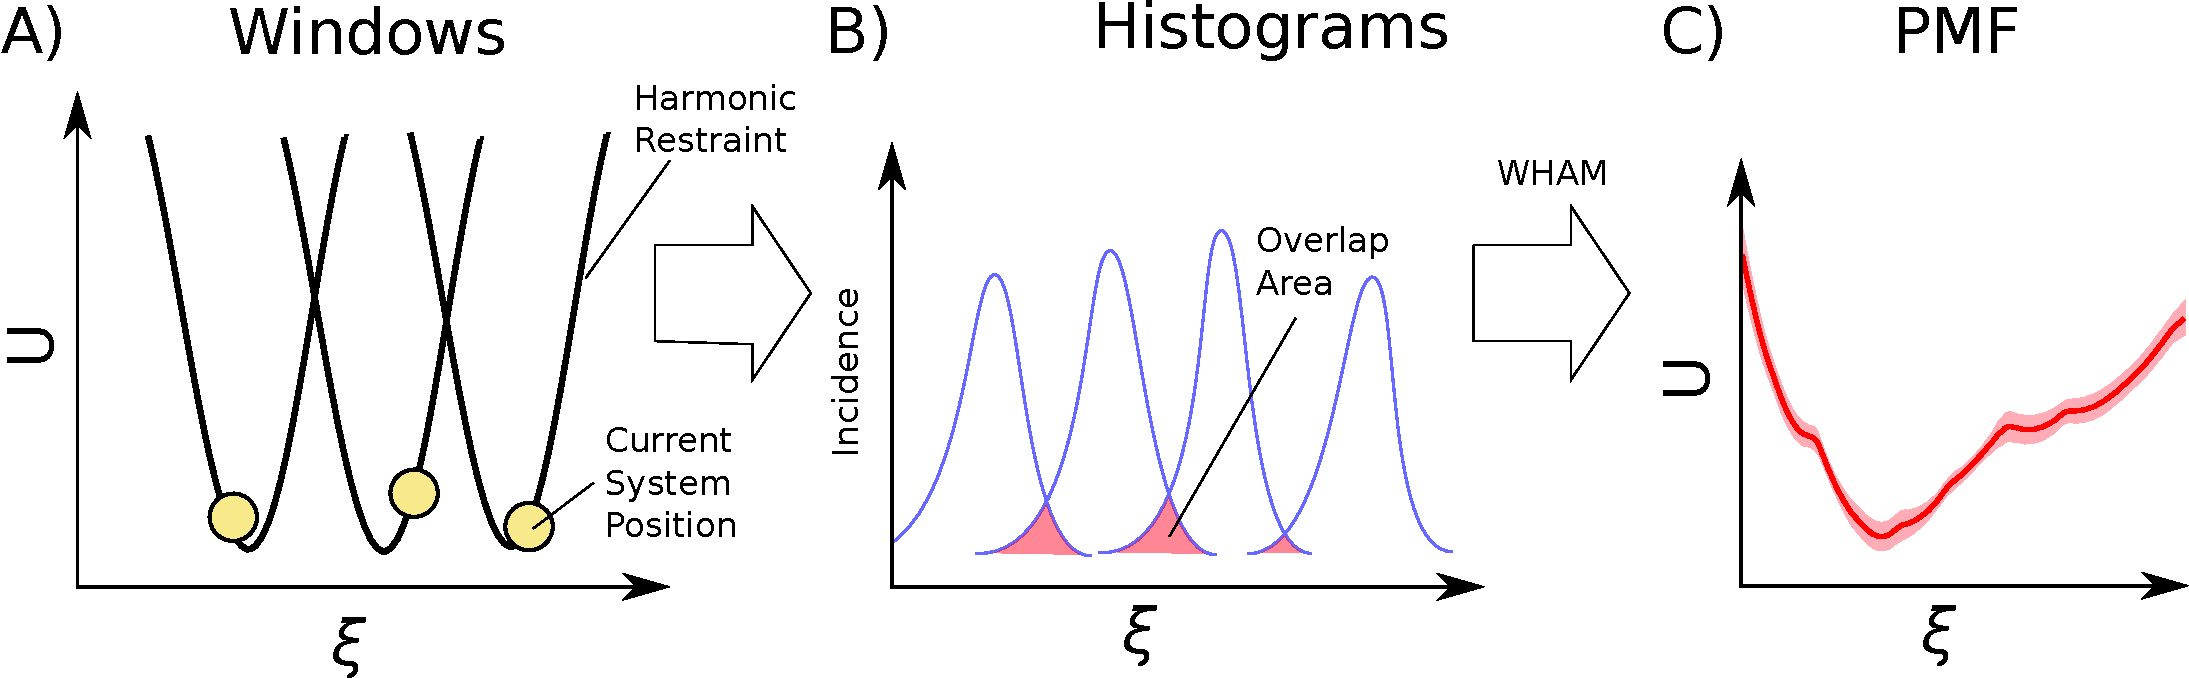
\includegraphics[width=\textwidth]{figures/umbrella_sampling.png.pdf}
	\end{center}
	\captionsetup{singlelinecheck = false, justification=raggedright}
	\caption[Illustration of Umbrella Sampling] {\textbf{Illustration of Umbrella Sampling}}{A) Several simulations are repeated with only one change. A bias  potential is added somewhere along the reaction coordinate $\xi$. B) The value of $\xi$ is recorded in each of the windows and then graphed as histograms. C) The Overlap in neighbouring histograms is integrated via the WHAM method to calculate the Potential of Mean Force. This gives us the energy landscape. Fluctuations in the overlap in the data can be used to estimate the error for the PMF. }
	\label{umbrella_sampling_illustration}
\end{figure}

This is possibly the most popular method of calculating the potential of a system along a reaction coordinate. The conceptual philosophy for the method is demonstrated in figure \ref{umbrella_sampling_illustration}. The molecular system is replicated in several "windows" and a harmonic $U_{biased}$ is added at several points along the collective variable $\xi$. Statistics are then collected in order to calculate the potential of mean force (PMF) and thus the energy landscape along between those windows.  

The functional form of $U_{bias}$ in umbrella sampling is then separated into $N$ windows. With the $n$th window having the biasing function:

\begin{equation}
	U_{b}^n = \frac{k^n_{\xi}}{2}(\xi(\bold{x}) - \xi_0^n)^2
	\label{umbrella_bias}
\end{equation}

Where $\xi_0^n$ is the equilibrium position of the restraint. $k_{\xi}^n$ is the strength of the harmonic restraint in the $n$th window. Typically this is the same in all windows. The more overlap between adjacent windows the more those windows are attracted to each other and the steeper the gradient of the free energy surface (FES) must be pushing those windows together. Conversely, when there is less overlap between adjacent windows it indicates the presence of a barrier in the energy landscape between those windows.

Umbrella sampling is extremly useful for calculating all sorts of experimental quantities and physiologically relevant proprties such as folding energies \cite{meshkin2017}, lipid binding \cite{domanski2017}, ion conduction \cite{zhu2012b}, and drug binding \cite{subramanian2019}. However, it is particularly sensetive to the choice of initial configuration and collective variable \cite{domanski2017}. The former issue is partiuclar to umbrella sampling because generally short runs are used since so many windows are spawned during the method, the simulations must be at equilibrium \textit{before} the method is attempted, and then sufficient statistics must be collected to average over any conformational changes orthogonal to the collective variable. In these ways, care must be taken when using this method to not introduce systematic error into the calculation \cite{you2019}. A deep knowledge of the molecular system under investigation can help aleviate some of these issues. 

\subsubsection{Weighted Histogram Average Method (WHAM)}
There a few candidates for calculating the PMF using the statistics calculated in umbrella sampling. The Weighted Histogram Average Method (WHAM)\cite{kumar1992}, Umbrella Integration (UI)\cite{kastner2005} and the Multistate Bennet Acceptance Ratio (MBAR)\cite{kim2012} are all used. We will breifly outline the mathematical formulation and estimation of errors of the WHAM method as it is more popular\cite{zhu2012}. Our explanation follows \cite{kastner2011} which covers the topic in more detail.

The method begins by dividing the sampled region into a set of $K$ histograms with $K$ being greater than the number of biased windows $N$.  The whole PMF can be estimated (poorly) from the $j$th biased histogram using 

\begin{equation}
	P_u^j(\xi) = P_b^j(\xi) \exp(\beta U_{b}^j (\xi)) \langle \exp(-\beta U_b^j (\xi))\rangle
\end{equation}

Where the $P(\xi)$  functions represent the probability density function calculated from samples collected at point $\xi$. The samples collected in each of these regions gives us an estimate of the PMF in the region according to equation \ref{}. These estimates are combined in a weighted sum using

\begin{equation}
	P_u(\xi) = \sum_j^K p_j(\xi)P_u^j (\xi)
\end{equation}

where the weights, $\sum_j^K p_j = 1$ are chosen such that the statistical error is minimised. This means an optimisation problem for the variance of the unbiased estimates

\begin{equation}
	\frac{\partial\text{Var} (P_u)}{\partial p_i}
\end{equation}

is solved to give the best estimates of the PMF given the data that has been collected. Essentially we are vertically shifting the estimates obtained in each of the histograms in order to minimise the error accross the PMF. By convention, we can estimate the error in the PMF by splitting up the statistics collected for the distributions of $P^b_i (\xi)$ and constructing PMFs from these independent samples. For example, we might have collected 100ns of data in each window, but we could construct 5 independent estimates for the PMF using 20ns blocks of trajectories. The Standard Error of the Mean (SEM) can then be used to estimate the error accross the surface \cite{gapsys2020}. By convention, an umbrella sampling calculation is said to have converged when the SEM from these independent samples has fallen below 1kcal/mol accross the PMF. Note that there may be sources of systematic error not captured by this criterion. 

\subsection{Metadynamics}
\begin{figure}
	\begin{center}
		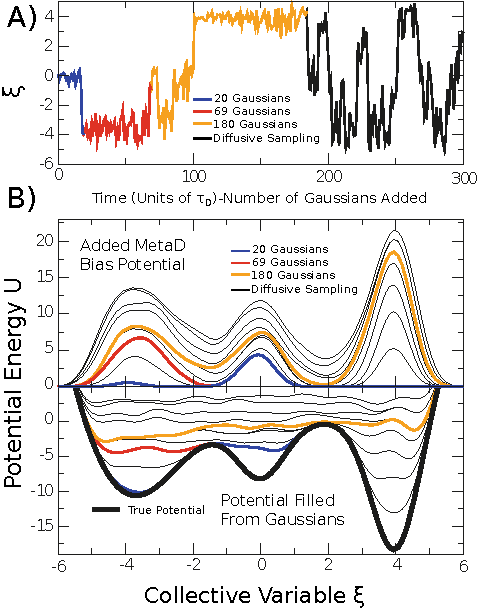
\includegraphics[width=0.7\textwidth]{figures/METAD_demonstration.pdf}
	\end{center}
	\captionsetup{singlelinecheck = false, justification=raggedright}
	\caption[Illustration of Metadynamics] {\textbf{Illustration of Metadynamics}}{A) The trajectory of a collective variable $\xi$ in a  metadynamics simulation. The blue region denotes the trajectory up to the time where 20 Gaussians have been deposited. After which the basin at $\xi=0$ has been filled. The red data points denote the time up until 69 Gaussians have been deposited, after which time the second basin at $\xi=-4$ has been adequately sampled. Finally the Orange data indicates that the 3rd basin at $\xi=4$ has been adequately sampled after which which time the system begins to sample $\xi$ diffusively and the simulation has converged. B) The upper pannel demonstrates the repulsive potentials that have been added to the simulation in order to drive it to new, unexplored regions. Multiplying the values of this function by $-1$  will be the estimate of the free energy surface. Note how in the lower panel the true potential the true potential energy surface is gradually filled by the added Gaussians functions.  Source\cite{bussi2020}}
	\label{umbrella_sampling_illustration}
\end{figure}

Metadynamics has proven to be a popular . The method relies on a time dependent form of $U_{bias}$ given by 

\begin{equation}
	U_{bias} (\xi,t) = \sum\limits_{\substack{t' = \tau_D, 2 \tau_D,... \\ t' < t}}  B \ \exp\bigg( - \frac{(\xi(t) - \xi(t') )^2}{2\sigma^2 }\bigg)
\end{equation}

This means the simulation is dropping virtual, repulsive Gaussian potentials at the positions along $\xi$ in order to encourage the simulation to sample regions of $\xi$ it has not visited already. The process is illustrated in figure \ref{METAD_demonstration}. The thermodynamic assumption of this method is that the deposition is done slow enough that the system remains at equilibrium, so the Gaussian height $B$ is chosen to be 0.1-0.2 kJ/mol in molecular systems. Usually, the Gaussian widths $\sigma$ are chosen to be the size of the variance in the unbiased measurements of $\xi$. 

The FES estimate at time $t$ from this method is simply the sum of all the gaussians we have added into the system inverted:  

\begin{equation}
	U_u (\xi,t)  =  \frac{1}{t_c-t} \int_{t_c}^t U_b(\xi,t) dt
\end{equation}

Formally, convergence is reached when the observed probability density is uniform across $\xi$. That is:
\begin{equation}
	P_b (\xi)= \frac{1}{V_\xi } 
	\label{convergence_criterion_metad}
\end{equation}

where $V_\xi$ is the volume of the phase space spanned by $\xi$. However, in practice the function $U_{bias}(\xi)$ is simply inspected at intervals for fluctuations about an average function \cite{sun2016}. 

There are many flavours of metadynamics. The most popular is well-tempered metadynamics which gradually reduces the Gaussian height $B$ as the simulation progresses\cite{barducci2008}. In theory, this guarantees convergence with vanishingly small error. However,this method requires an estimate of how long the simulation will take to converge. There is also infrequent metadynamics which can be used to estimate the diffusion profile along $\xi$\cite{tiwary2013}\cite{tiwary2016}\cite{salvalaglio2014}.  

A useful feature of the Metadynamics method is that it can be linearly sped up with the number of parallel simulations. This is known as multiple walker metadynamics\cite{raiteri2006}. Since we are simply attempting to sample from the same potential $U_{MM}$ up to a desired time, until the criterion in equation \ref{convergence_criterion_metad} is met, we can speed this process up by running simulations in parallel and adding Gaussian to the same $U_{bias}$ function.

Conceptually, metadynamics performs the same role as umbrella sampling and should in theory produce the same results in the same system with the same collective variable $\xi$. However, it has some specific contexts where it outperforms umbrella sampling. This method is more suited to an exploration of free energy space where it can intelligently explore regions which are poorly sampled, whereas umbrella sampling requires some foreknowledge of the surface being investigated in order to guess which parts of the landscape require more sampling. However, metadynamics can be very difficult converge. A good indicator of such systematic errors are the presence of unphysically large barriers, indicating that there are orthogonal degrees of freedom not sampled along $\xi$ which might correspond to a minimum energy pathway. These barriers will eventually come down in the infinite sampling limit but many barrier crossings will need to be observed. 

\section{Short Comings of Classical MD}
The short comings of classical molecular dynamics fall into two classes whose solutions stand opposed to one another. These are the accuracy of the chemical forcefields outlined in section \ref{forcefields_review} and the inability of modern computers to deliver enough samples of the energy landscape to collect sufficient statistics for rigorous conclusions. The issue is that, as the above physical formulation might indicate in section \ref{born-oppenheimer}. The more accurate the forcefields, the more computationally expensive calculations in its potential will be. And so the solutions to the two are constantly in tension with one another. In the next section we will explore the current efforts to bring solutions to both problems.

\subsubsection{The Problem with Forcefields}
These approximations are not without a cost to accuracy. In certain situations, many of which are biologically relevant, it has been shown that quantum effects such as polarisation play an important role in the dynamics of the system. This has been demonstrated in the literature for Gramicidin where polarisable forcefields are able to more accurately reproduce the experimental results of current\cite{ngo2021}.

The other context where polarisation is important to consider are on divalent ions. Here, the solvation energy is underestimated due to the consistent lack of polarisation, making investigations of these biologically important chemical species difficult.

However, for most situations, particularly those involving bulk water and protein motions Molecular Dynamics is proving to be an invaluable tool for investigating the properties of biological systems \cite{hollingsworth2018}. Sadly, it should be kept in mind that classical MD is not able to simulate any chemistry such as forming and breaking or the change a change in protonation state. Such interactions require considerations of Quantum Mechanics which are computationally expensive.

There are several efforts to correct address some of the above issues. These include the inclusion of the effects of polarisation, the most popular methods at the moment being adding a massless drude oscillator as an extra bead to atoms as in the CHARMM drude forcefields, championed by the Mackerell lab and the use of forcefields such as AMOEBA which explicitly calculate the dipole and quadrupole moments of each atom. These both substantially increase computational cost but have displayed much better agreement with experiments in biological systems where classical forcefields have been shown to fail \cite{ngo2021}\cite{li2017}\cite{shi2013}. 

Ultimately, the functional form in equation \ref{CHARMM_effective_potential_eq} used by classical forcefields does not have sufficient degrees of freedom to address all possible chemical contexts. Careful consideration must always be given to whether the forcefield is being used in a faithful way to the situations it was intended to accurately represent. So long as the user is aware of the situations where a given forcefield falls short, classical forcefields can be a powerful tool for the study of molecular systems.

\subsubsection{The Problem with Sampling}

To physicists the sampling is the more intuitive. Collecting sufficient statistics about the system of interest is difficult and comes at both a computational and human cost. Even though computers have sped up exponentially for the last 50 years we are still orders of magnitude from being able to reach the time scales of many biological processes, as displayed in table \ref{timescales}.

The slow time step demanded in classical MD due to the fast motions of certain atomic groups such as hydrogen is fundamentally at odds with the time scales of many important biological processes such as drug binding or protein folding which occur on the time scale of  milliseconds or seconds.  

Methods are now emerging which intelligently drive the simulation toward regions unexplored in the collective variable space by unbiased simulations. For some time the field has used steered methods or adaptive sampling methods such as Umbrella Sampling or Metadynamics to drive the simulation toward sections of the energy landscape which are under sampled. These methods universally rely on a choice of collective variable which closely corresponds to a slow degree of freedom. Such a choice is not usually simple. In the case of ion channels one may rationally choose the placement of the ion along the conduction pathway as the collective variable but the choice is less obvious in the case of more global conformational changes.

The success of simulations at the millisecond timescale by D.E Shaw research suggest that we are in reach of an exciting area in biological research \cite{lindorff-larsen2016}. Enhanced sampling methods will be able to routinely reach motions that occur on these time scales and as software and hardware improve we will be able to push further for larger systems. This indicates that the enhanced sampling approach holds great promise.

The advances we are seeing at the moment which I find exciting are the use of machine learning methods to tease out these degrees of freedom in order to accelerate them with already established free energy methods. These have the potential to uncover new drug binding pockets and revolutionise our understanding of biomolecular systems. 

\section{Conclusion}
It is hoped that the preceding chapter can serve as a roadmap for any physicists interested in beginning to study the exciting field of biophysics. The information in each section should serve to help you understand the foundations of what you are trying to simulate. The next steps would be to learn more about the molecular biology and biochemistry of macromolecules so they can better understand the wet, messy dance occurring inside cells. There is a lot to learn and the barrier to entry can seem daunting. The reader is encouraged to join mailing lists and other forums where the thriving computational chemistry and computational biophysics communities communicate. Send cold emails asking for help when you are stuck, read software manuals. No individual who has studied a specific discipline has the skills necessary to pick up biomolecular simulation software and begin using it. Physicists lack the understanding of the biology and the chemistry involved in the biological systems, while chemists and biologists will lack an understanding of the deep mathematics that has gone into producing highly accurate simulations of molecular systems. The reader is encouraged to seek out members of other disciplines such as cell biologists and protein chemists and learn how they do what they do and how their skills and knowledge can compliment each other.
